\documentclass[answers]{exam} % Clase para exámenes con respuestas
\usepackage[english,spanish]{babel} % Soporte para inglés y español
\usepackage[autostyle]{csquotes} % Manejo de citas
\usepackage{amsmath, amssymb} % Paquetes para matemáticas avanzadas
\usepackage{graphicx} % Inclusión de gráficos
\usepackage{enumitem} % Personalización de listas enumeradas
% \usepackage[letterpaper,top=2cm,bottom=2cm,left=3cm,right=3cm,marginparwidth=1.75cm]{geometry} % Configuración de márgenes
\usepackage[colorlinks=true, allcolors=blue]{hyperref} % Enlaces con color

\renewcommand{\solutiontitle}{\noindent\textbf{Respuesta:}\par\noindent} % Personalización del título de respuestas
\renewcommand{\familydefault}{\sfdefault}

\pagestyle{headandfoot}
\firstpageheader{}{}{} 
\runningheader{}{}{}
\firstpagefooter{}{}{}
\runningfooter{}{}{}

\begin{document}

\large\textbf{Funciones:}
\[
	f(x) =
	\begin{cases}
		\dfrac{x^2 - 1}{x+1}, & \text{si } x \leq 1   \\
		\\
		\dfrac{1-x}{x},       & \text{si }1< x \leq 3 \\
		\\
		\dfrac{2x}{x-5},      & \text{si } x > 3
	\end{cases}
	\text{ en } x = 1 \text{ y en } x =3
\]
\[
	g(x)=\dfrac{x^2}{x-1}
\]\\[1em]

\vspace{1cm}
\large\textbf{Procedimiento:}\\

\begin{questions}

	% Question 1
	\question \large\textbf{Graficar la función f(x) utilizando el GeoGebra.}

	\begin{minipage}{\textwidth}
		\centering
		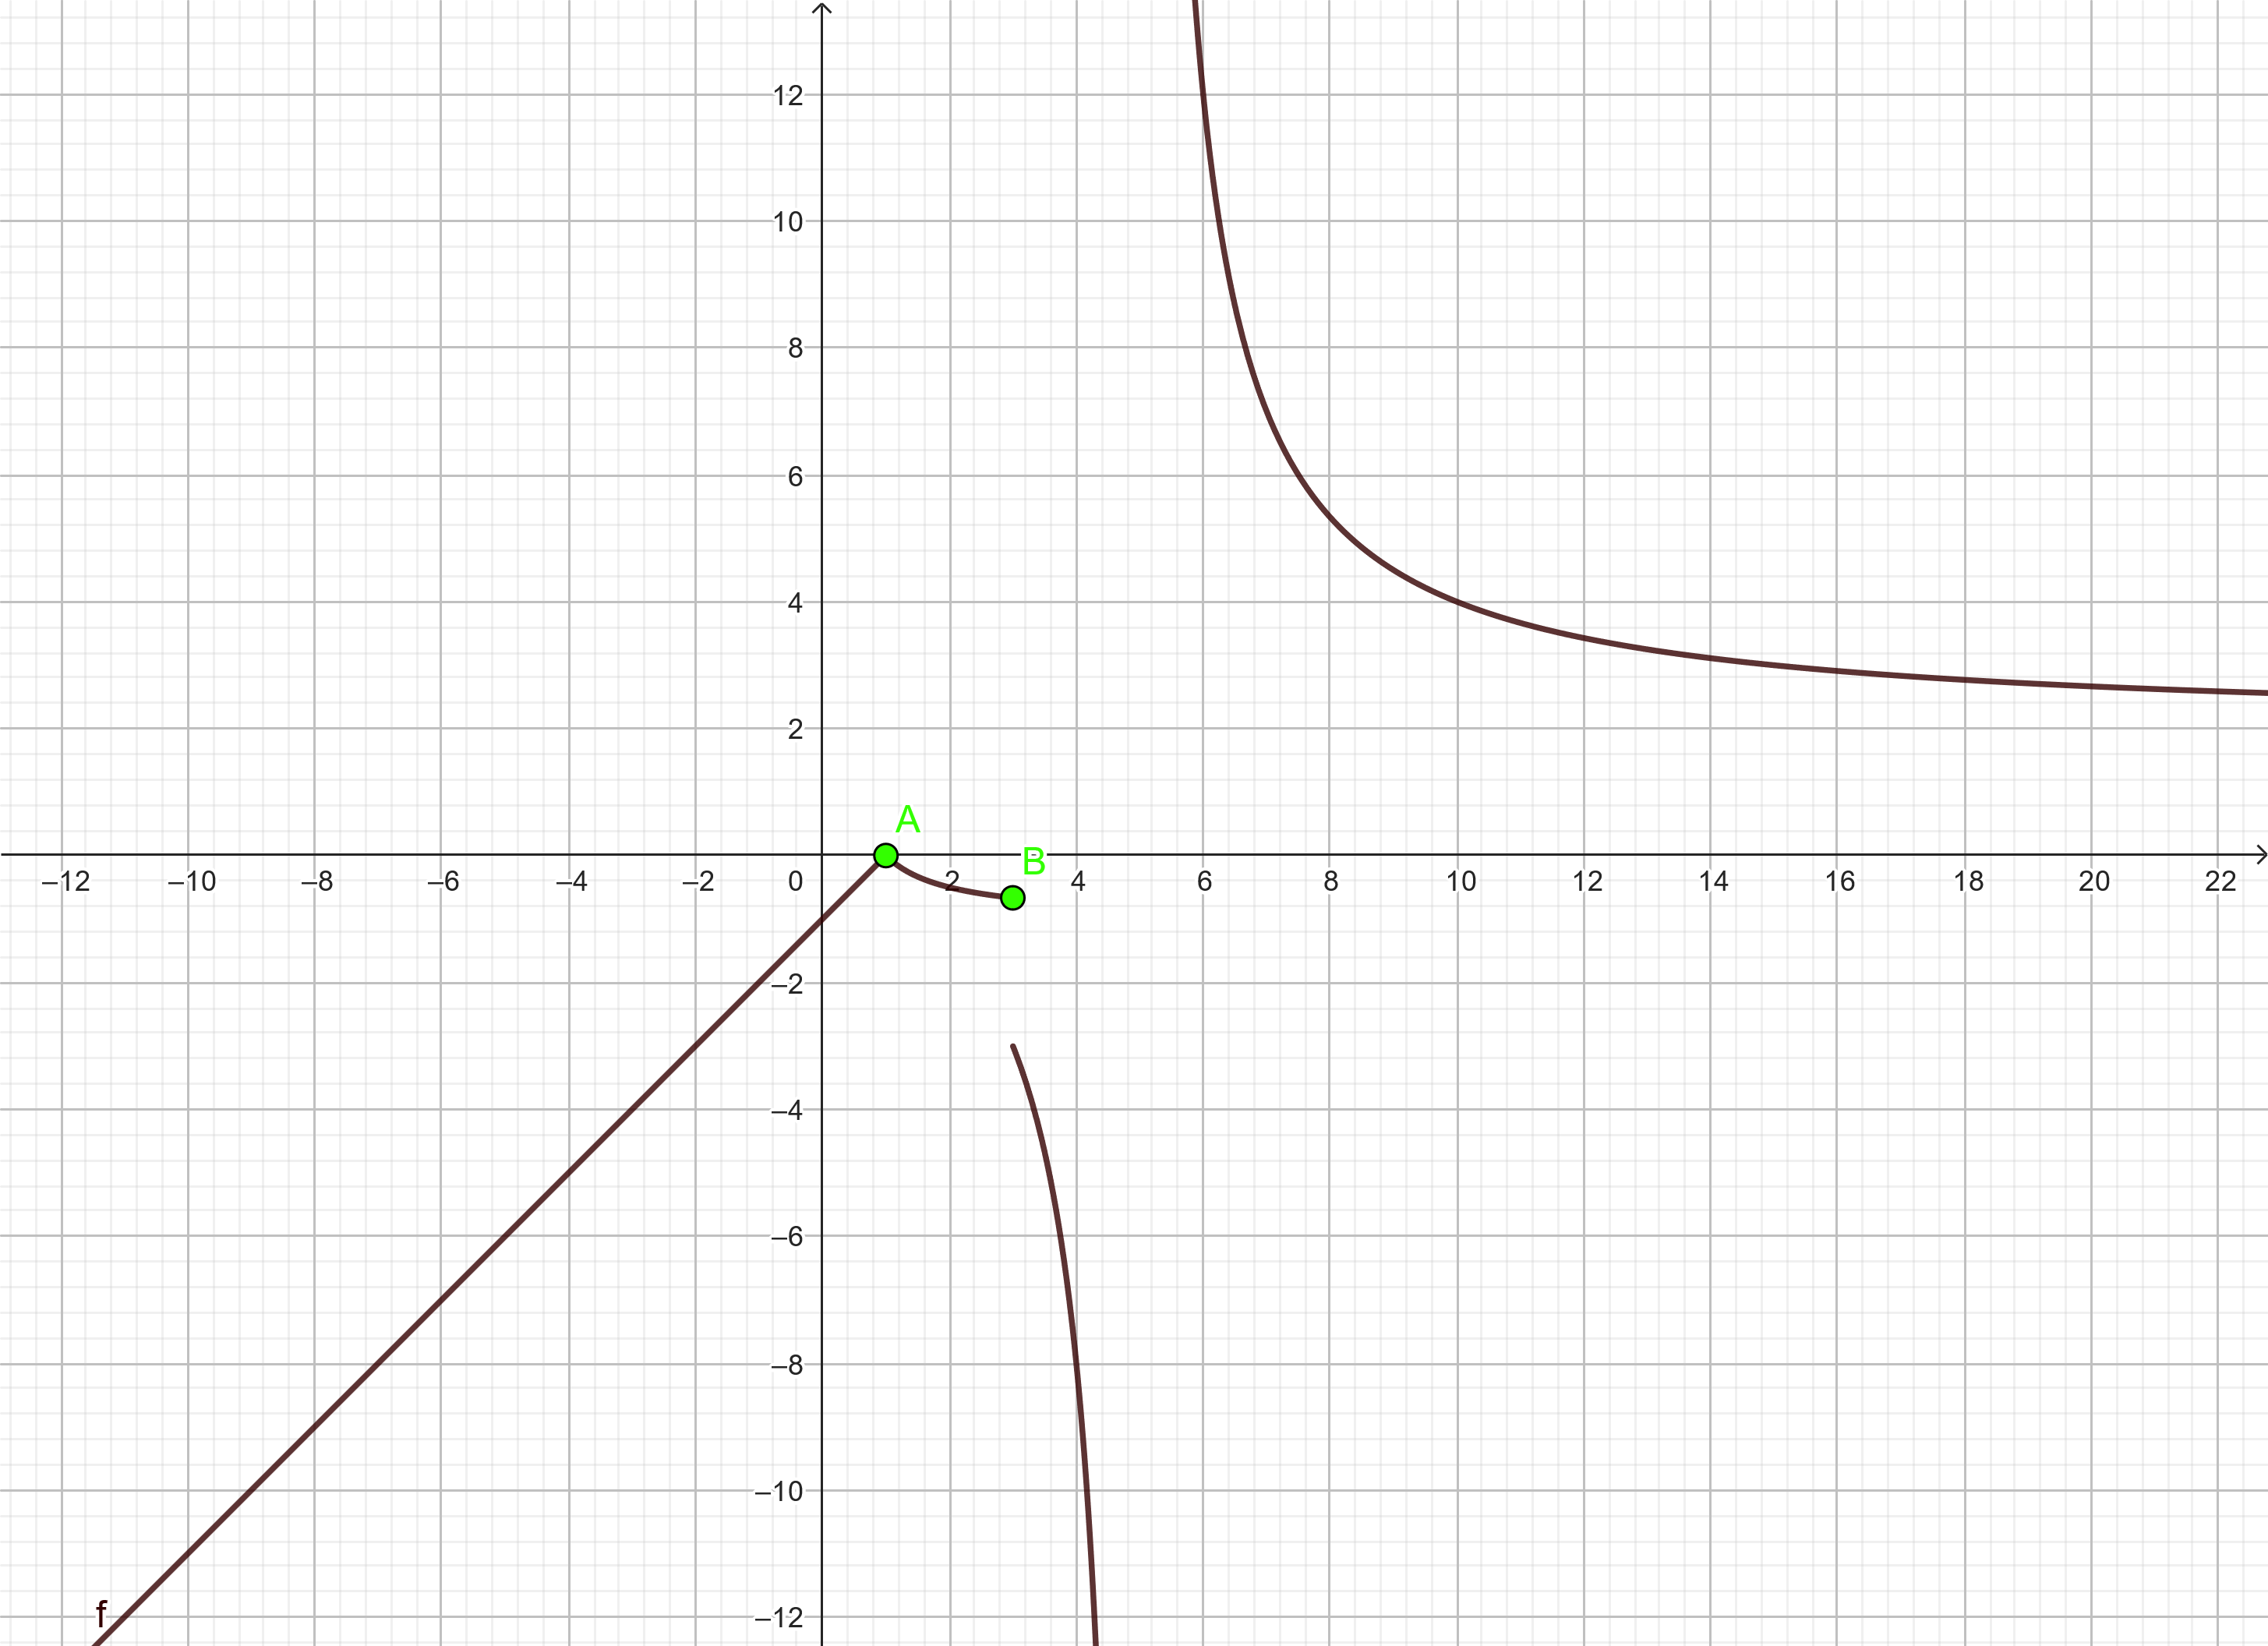
\includegraphics[width=0.9\textwidth]{public/g1.png}\\
	\end{minipage}

	\vspace{0.5cm}
	\newpage
	% Question 2
	\question \large\textbf{Del gráfico determine si la función es continua en los puntos dados.}

	\begin{solution}
		Para determinar si la función \( f(x) \) es continua en los puntos dados \( x = 1 \) y \( x = 3 \), evaluamos la continuidad en cada uno de estos puntos:

		1. En \( x = 1 \):

		- Evaluamos el límite cuando \( x \) se acerca a 1 por la izquierda (\( x \leq 1 \)):

		\[
			\lim_{{x \to 1^-}} f(x) = \lim_{{x \to 1^-}} \frac{x^2 - 1}{x+1} = \frac{1^2 - 1}{1+1} = \frac{0}{2} = 0
		\]

		- Evaluamos el valor de la función en \( x = 1 \):

		\[
			f(1) = \frac{1^2 - 1}{1+1} = \frac{0}{2} = 0
		\]

		- Evaluamos el límite cuando \( x \) se acerca a 1 por la derecha (\( 1 < x \leq 3 \)):

		\[
			\lim_{{x \to 1^+}} f(x) = \lim_{{x \to 1^+}} \frac{1 - x}{x} = \frac{1 - 1}{1} = 0
		\]

		$\implies$Por lo tanto, la función es continua en \( x = 1 \)  porque:
		\[
			\lim_{{x \to 1^-}} f(x) = f(1) = \lim_{{x \to 1^+}} f(x)
		\]

		2. En \( x = 3 \):

		- Evaluamos el límite cuando \( x \) se acerca a 3 por la izquierda (\( 1 < x \leq 3 \)):

		\[
			\lim_{{x \to 3^-}} f(x) = \lim_{{x \to 3^-}} \frac{1 - x}{x} = \frac{1 - 3}{3} = -\frac{2}{3}
		\]

		- Evaluamos el límite cuando \( x \) se acerca a 3 por la derecha (\( x > 3 \)):

		\[
			\lim_{{x \to 3^+}} f(x) = \lim_{{x \to 3^+}} \frac{2x}{x-5} = \frac{2 \cdot 3}{3 - 5} = \frac{6}{-2} = -3
		\]

		$\implies$Por lo tanto, la función no es continua en \( x = 3 \)  porque:

		\[
			\lim_{{x \to 3^-}} f(x) \neq \lim_{{x \to 3^+}} f(x)
		\]
		$\implies$Por lo tanto, la función \( f(x) \) es discontinua en \( x = 3 \).
	\end{solution}


	\vspace{0.5cm}

	% Question 3
	\question \large\textbf{Si es discontinua, diga de qué tipo es:}
	\begin{solution}
		Para determinar si la discontinuidad en \( x = 3 \) es evitable o inevitable, debemos considerar lo siguiente:


		\[
			\lim_{{x \to 3^-}} f(x) = \lim_{{x \to 3^-}} \frac{1 - x}{x} = \frac{1 - 3}{3} = -\frac{2}{3}
		\]


		\[
			\lim_{{x \to 3^+}} f(x) = \lim_{{x \to 3^+}} \frac{2x}{x-5} = \frac{2 \cdot 3}{3 - 5} = \frac{6}{-2} = -3
		\]

		En este caso, los límites laterales son diferentes (\(-\frac{2}{3}\) y \(-3\)), lo que significa que no es posible ajustar el valor de la función en \( x = 3 \) para igualar los límites.\\[10pt]
		$\implies$Por lo tanto, la discontinuidad en \( x = 3 \) es \textbf{inevitable}.


	\end{solution}



	\vspace{0.5cm}

	% Question 4
	\question \large\textbf{Encuentre analíticamente la(s) asíntotas que tiene la función g(x)}
	\begin{solution}
		Para encontrar las asíntotas de la función \( g(x) = \dfrac{x^2}{x-1} \), analizamos los siguientes tipos de asíntotas:

		1. Asíntotas verticales:

		Las asíntotas verticales ocurren donde el denominador se hace cero y la función tiende a infinito. Para \( g(x) \), esto ocurre cuando \( x - 1 = 0 \):

		\[
			x = 1
		\]

		$\implies$Por lo tanto, la función tiene una asíntota vertical en \( x = 1 \).

		2. Asíntotas horizontales:

		Las asíntotas horizontales se encuentran al evaluar el límite de la función cuando \( x \) tiende a \( \pm\infty \). Para \( g(x) \):

		\[
			\lim_{{x \to \infty}} \frac{x^2}{x-1} = \lim_{{x \to \infty}} \frac{x^2}{x} \cdot \frac{1}{1 - \frac{1}{x}} = \lim_{{x \to \infty}} x \cdot 1 = \infty
		\]

		\[
			\lim_{{x \to -\infty}} \frac{x^2}{x-1} = \lim_{{x \to -\infty}} \frac{x^2}{x} \cdot \frac{1}{1 - \frac{1}{x}} = \lim_{{x \to -\infty}} x \cdot 1 = -\infty
		\]

		$\implies$Por lo tanto, la función no tiene asíntotas horizontales ya que tiende a infinito tanto en \( x \to \infty \) como en \( x \to -\infty \).

		3. Asíntotas oblicuas:

		Las asíntotas oblicuas se encuentran cuando la función no tiene asíntotas horizontales, y se determinan mediante la división larga del numerador por el denominador. Realizamos la división de \( x^2 \) por \( x-1 \):

		\[
			\frac{x^2}{x-1} = x + \frac{x}{x-1}
		\]

		A medida que \( x \to \infty \) o \( x \to -\infty \), el término \( \frac{x}{x-1} \) tiende a 1. Entonces, la asíntota oblicua es:

		\[
			y = x + 1
		\]

		$\implies$Por lo tanto, la función \( g(x) = \frac{x^2}{x-1} \) tiene una asíntota vertical en \( x = 1 \) y una asíntota oblicua \( y = x + 1 \).
	\end{solution}


	\vspace{0.5cm}

	% Question 5
	\question \large\textbf{Utilizando el GeoGebra, grafique la(s) asíntotas encontradas en el numeral anterior.}
	\begin{minipage}{\textwidth}
		\centering
		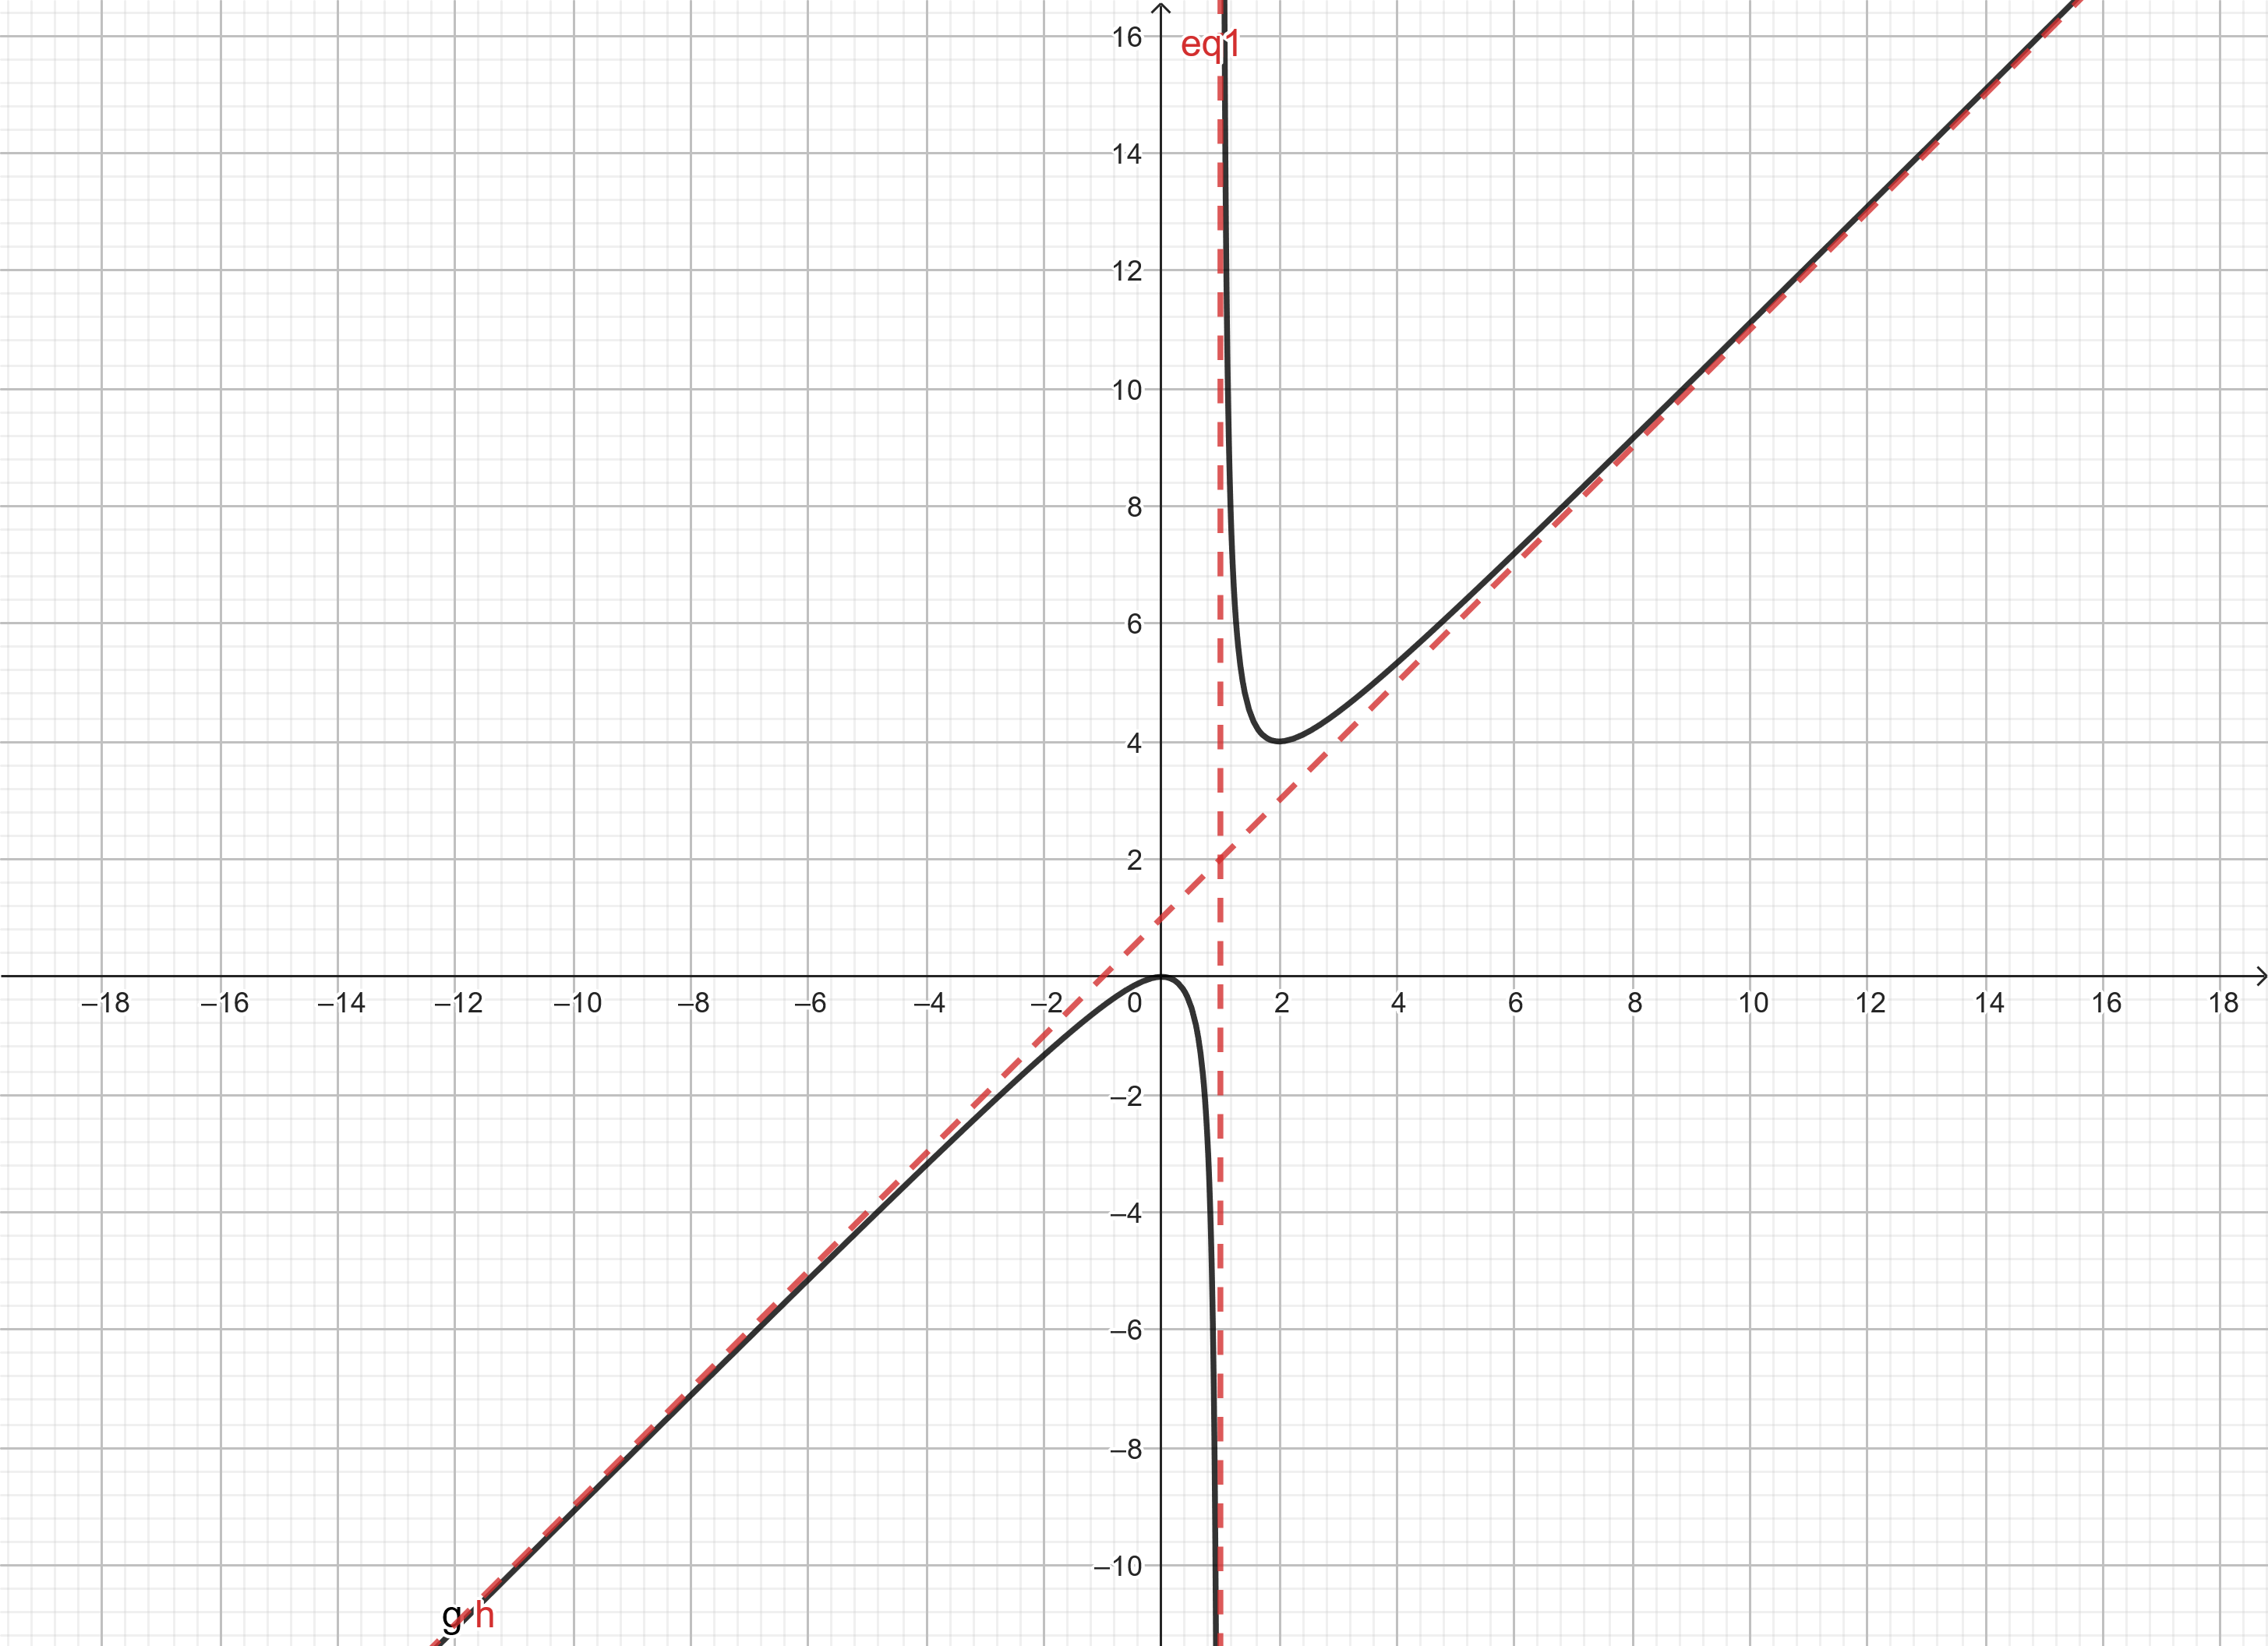
\includegraphics[width=0.9\textwidth]{public/g2.png}\\
	\end{minipage}


\end{questions}

\end{document}
